%%%%%%%%%%%%%%%%%%%%%%%%%%%%%%%%%%%%%%%%%
% Name of presentation: File formatting
% Code: it2r
% Content & presentation author: Daniel Adámek
% Project is used as teaching material on SPSE Jecna, Praha
%
% Beamer Presentation
% LaTeX Template
% Version 1.0 (10/11/12)
%
% License:
% CC BY-NC-SA 3.0 (http://creativecommons.org/licenses/by-nc-sa/3.0/)
%
%%%%%%%%%%%%%%%%%%%%%%%%%%%%%%%%%%%%%%%%%

\documentclass{beamer}

\definecolor{FMTUL}{RGB}{234, 118, 3}
\mode<presentation> {
\usecolortheme[named=FMTUL]{structure}
\usetheme{Rochester}

\setbeamertemplate{footline}[page number] % To replace the footer line in all slides with a simple slide count uncomment this line

\setbeamertemplate{navigation symbols}{} % To remove the navigation symbols from the bottom of all slides uncomment this line
}

\uselanguage{czech}
\usepackage{graphicx} % Allows including images
\usepackage{booktabs} % Allows the use of \toprule, \midrule and \bottomrule in tables
\usepackage[czech]{babel}
\usepackage[utf8x]{inputenc}
\usepackage{amsmath,tikz}
\usepackage{xcolor}
\usepackage{multicol}
\graphicspath{{./Images/}}

%----------------------------------------------------------------------------------------
%	TITLE PAGE
%----------------------------------------------------------------------------------------

\title[Titulek]{ALG1 - Semestrální práce}
\author{Daniel Adámek}
\institute[Technická univerzita v Liverci]
{}
\date{\today} % Date, can be changed to a custom date
\newcommand{\rlight}[1]{%
    \ooalign{\hss\makebox[0pt]{\fcolorbox{red!80}{red!40}{$#1$}}\hss\cr\phantom{$#1$}}%
}
\newcommand{\glight}[1]{%
    \ooalign{\hss\makebox[0pt]{\fcolorbox{green!80}{green!40}{$#1$}}\hss\cr\phantom{$#1$}}%
}
\setlength{\columnseprule}{0pt}

\begin{document}

\begin{frame}
\titlepage % Print the title page as the first slide
\end{frame}

%----------------------------------------------------------------------------------------
%	PRESENTATION SLIDES
%----------------------------------------------------------------------------------------
\section{Zadání}
\begin{frame}
\frametitle{Zadání}
    \textbf{Zadání č. 21:} \\
    Vytvořte program, který po zadání rozměru čtvercové matice načte 2 data matice a vyhodnotí, zda-li není jedna
    tranformací - rotace druhé matice, případně o kolik stupňů.
\end{frame}
\begin{frame}
\frametitle{Algoritmus validace rotace matic}
    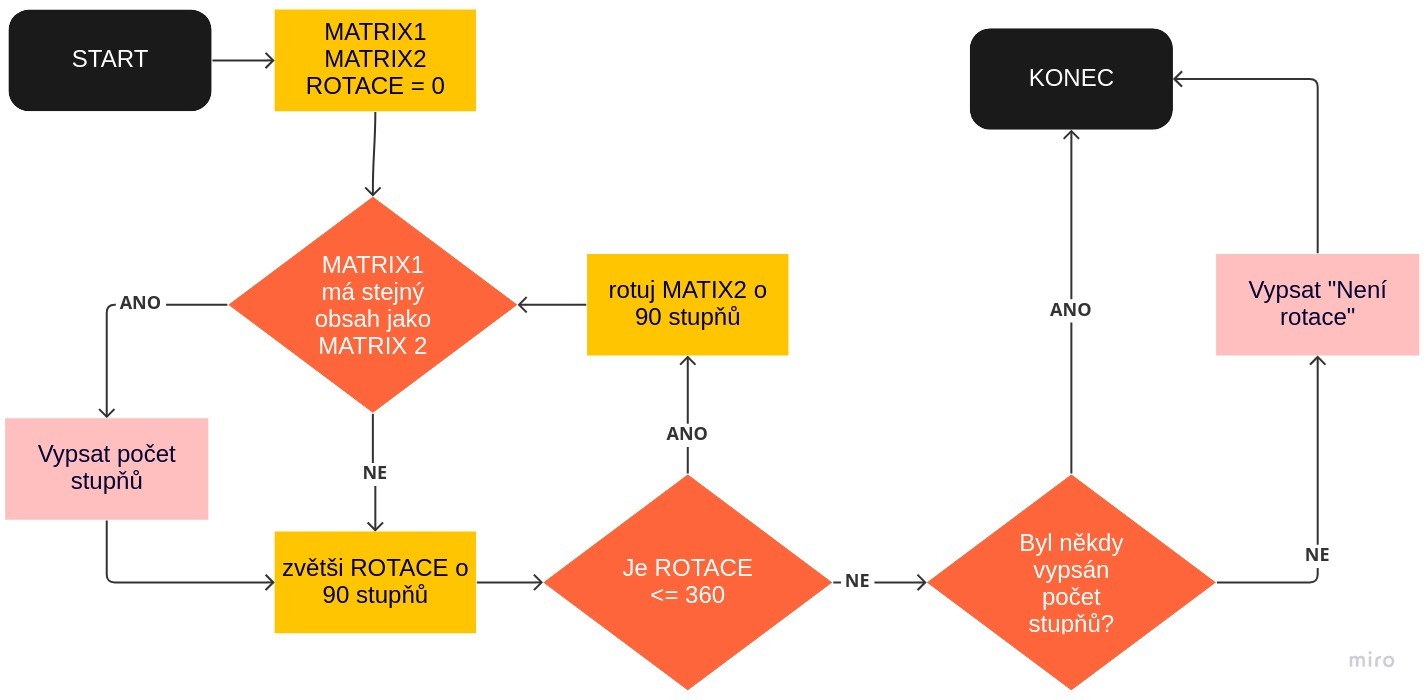
\includegraphics[scale=0.215]{alg1-flowchart}
\end{frame}
\begin{frame}
    \frametitle{Rotace matice o 90 stupňů \small{po směru hodinových ručiček}}
    
\includegraphics[scale=0.12]{alg1-rotate-flowchart}
\end{frame}
\begin{frame}
    \frametitle{Rotace matice o 90 stupňů \small{postup}}
    Mějme matici $2\times2$
    \[
    \begin{pmatrix}
        1 & 2\\
        3 & 4
    \end{pmatrix}
    \]
    Převrátíme pořadí řádků
    \[
    \begin{pmatrix}
        \glight{1} & \glight{2}\\
        \rlight{3} & \rlight{4}
    \end{pmatrix}
    \rightarrow
    \begin{pmatrix}
        \rlight{3} & \rlight{4}\\
        \glight{1} & \glight{2}
    \end{pmatrix}
    \]
    Transponujeme matici
    \[
    \begin{pmatrix}
        \rlight{3} & \rlight{4}\\
        \glight{1} & \glight{2}
    \end{pmatrix}
    \rightarrow
    \begin{pmatrix}
        \rlight{3} & \glight{1}\\
        \rlight{4} & \glight{2}
    \end{pmatrix}
    \]
    \[
    \begin{pmatrix}
        3 & 1\\
        4 & 2
    \end{pmatrix}
    \]
\end{frame}
\begin{frame}
\frametitle{Nejzajímavější část kódu (rotace)}
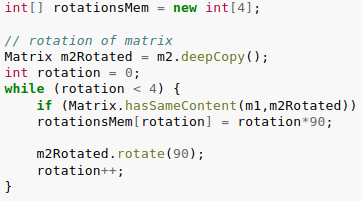
\includegraphics[scale=0.6]{java-code}

\end{frame}
\begin{frame}
    \frametitle{JUnit testování}
    \begin{multicols}{3}
        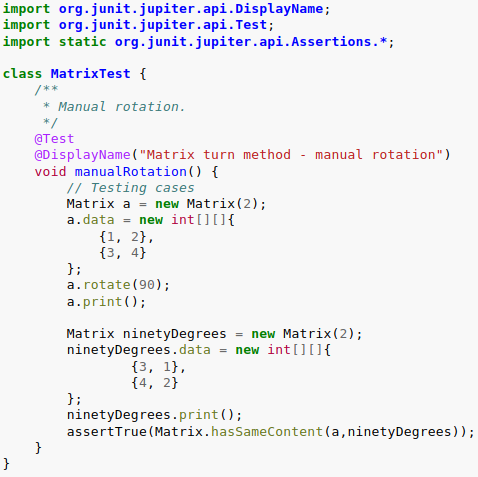
\includegraphics[scale=0.4]{alg1-unit-code}
        \columnbreak

        \columnbreak
        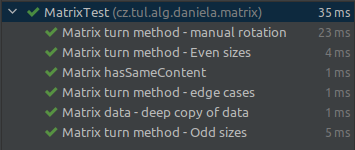
\includegraphics[scale=0.3]{alg1-unit-tests}
    \end{multicols}
\end{frame}
\begin{frame}
    \frametitle{Testování programu}
    \begin{multicols}{4}
    \textbf{Vstup}\\
    \small{3\\
    1 2 3\\
    4 5 6\\
    7 8 9\\
    7 4 1\\
    8 5 2\\
    9 6 3\\
    3\\
    1 2 3\\
    4 5 6\\
    7 8 9\\
    3 6 9\\
    2 5 8\\
    1 4 7\\
    \columnbreak
    3\\
    1 2 3\\
    4 5 6\\
    7 8 9\\
    1 4 7\\
    2 5 8\\
    3 6 9\\
    -1}

    \columnbreak
    \textbf{Výstup}\\
    \small{
    Rozměr matic\\
    První matice\\
    Druhá matice\\
    Rotace 270\\

    Rozměr matic\\
    První matice\\
    Druhá matice\\
    Rotace 90\\

    Rozměr matic\\
    První matice\\
    Druhá matice\\
    Není rotací\\

    Rozměr matic}

    \columnbreak
    \textbf{Reference}\\
    \small{
    Rozměr matic\\
    První matice\\
    Druhá matice\\
    Rotace 270\\

    Rozměr matic\\
    První matice\\
    Druhá matice\\
    Rotace 90\\

    Rozměr matic\\
    První matice\\
    Druhá matice\\
    Není rotací\\

    Rozměr matic}

    \end{multicols}

    \small{Záznam o testu v složce \textit{/test}}
\end{frame}

\end{document} 
